\chapter{单级放大电路的设计与仿真}%
\label{cha:单级放大电路的设计与仿真}

\section{实验目的}%
\label{sec:\arabic{chapter}实验目的}

\begin{enumerate}
	\item 设计一个分压偏置的单管电压放大电路,要求电压增益大于50,输出电阻设计在\SI{5}{\kohm}以内,带宽大于\SI{500}{\kHz}。
	\item 已知供电电源为\SI{12}{\V},三极管型号BC817-16,负载电阻为\SI{20}{\kohm}。输入信号为:频率为\SI{10}{\kHz},峰值\SI{1}{\mV}$ \sim $\SI{5}{\mV}的正弦信号。
	\item 放大器指标测量:在放大器输入端接入正弦信号,调节电路静态工作点(调节偏置电阻),观测电路输出信号,使得输出波形不失真。在此状态下测试:

		\begin{enumerate}
			\item 电路静态工作点值;
			\item 三极管的输入、输出特性曲线和$ \beta $、$ r_\mathrm{be} $、$ r_\mathrm{ce} $值 ;
			\item 利用示波器得到输出波形,求出该放大电路的放大倍数;
			\item 利用交流扫描分析(ACAnalysis/ACSweep)画出电路电压增益的幅频特性和相频特性;
			\item 利用交流扫描分析画出输出变量为$ R_\mathrm{i} = \dfrac{V_\mathrm{i}}{I_\mathrm{i}} $的频率特性曲线图,读出电路工作频率\SI{10}{\kHz}时的值,从而得到电路输入电阻的值;
			\item 将信号源$ V_\mathrm{i} $短路,负载电阻用一个信号源$ V_\mathrm{T} $替代。再进行交流扫描分析,画出输出变量$ R_\mathrm{o} = \dfrac{V_\mathrm{T}}{I_\mathrm{T}} $,读出电路对应工作频率下的值,从而得到电路输出电阻的值。
		\end{enumerate}

	\item 观察失真波形:调节电路静态工作点(调节偏置电阻),观察电路出现饱和失真和截止失真的输出信号波形,并测试对应的静态工作点值。
\end{enumerate}

\section{实验要求}%
\label{sec:\arabic{chapter}实验要求}

\begin{Exercise}
	给出单级放大电路原理图。
\end{Exercise}

\begin{Answer}
	单级放大电路原理图见图\ref{fig:单级放大电路原理图}。
\end{Answer}

\begin{Exercise}
	电路工作在不失真状态下:

	\begin{enumerate}
		\item 给出三极管静态工作点的测量值;
		\item 给出测试三极管在该工作点下的值$ \beta $、$ r_\mathrm{be} $、$ r_\mathrm{ce} $的实验图和测试结果;
		\item 给出输出波形图,求出放大倍数,并与理论计算值进行比较;
		\item 给出电路的幅频和相频特性图,并得出下限截止频率$ f_\mathrm{L} $、上限截止频率$ f_\mathrm{H} $以及带宽BW值;
		\item 给出输入电阻的幅频特性图,求出工作频率下输入电阻的测试结果,并和理论计算值进行比较;
		\item 给出测量输出电阻的实验图,以及输出电阻的幅频特性图,求出工作频率下输出电阻的测试结果,并和理论计算值进行比较。
	\end{enumerate}

\end{Exercise}

\begin{Answer}
	单级放大电路失真参数见表\ref{tab:单级放大电路失真指标},三极管参数见表\ref{tab:三极管参数},频率响应见图\ref{fig:单级放大电路增益},输入电阻和输出电阻见章节\ref{sub:\arabic{chapter}误差分析}。
\end{Answer}

\begin{Exercise}
	给出电路饱和失真和截止失真时输出电压的波形图。并给出两种状态下三极管的静态工作点值。分析出现失真原因。
\end{Exercise}

\begin{Answer}
	饱和失真波形图见图\ref{fig:单级放大电路饱和失真},截止失真波形图见图\ref{fig:单级放大电路截止失真}。静态工作点见表\ref{tab:单级放大电路参数},失真原因见章节\ref{sub:\arabic{chapter}仿真结果}。
\end{Answer}

\section{实验步骤}%
\label{sec:\arabic{chapter}实验步骤}

\subsection{设计电路}%
\label{sub:\arabic{chapter}设计电路}

\begin{figure}[H]
	\centering
	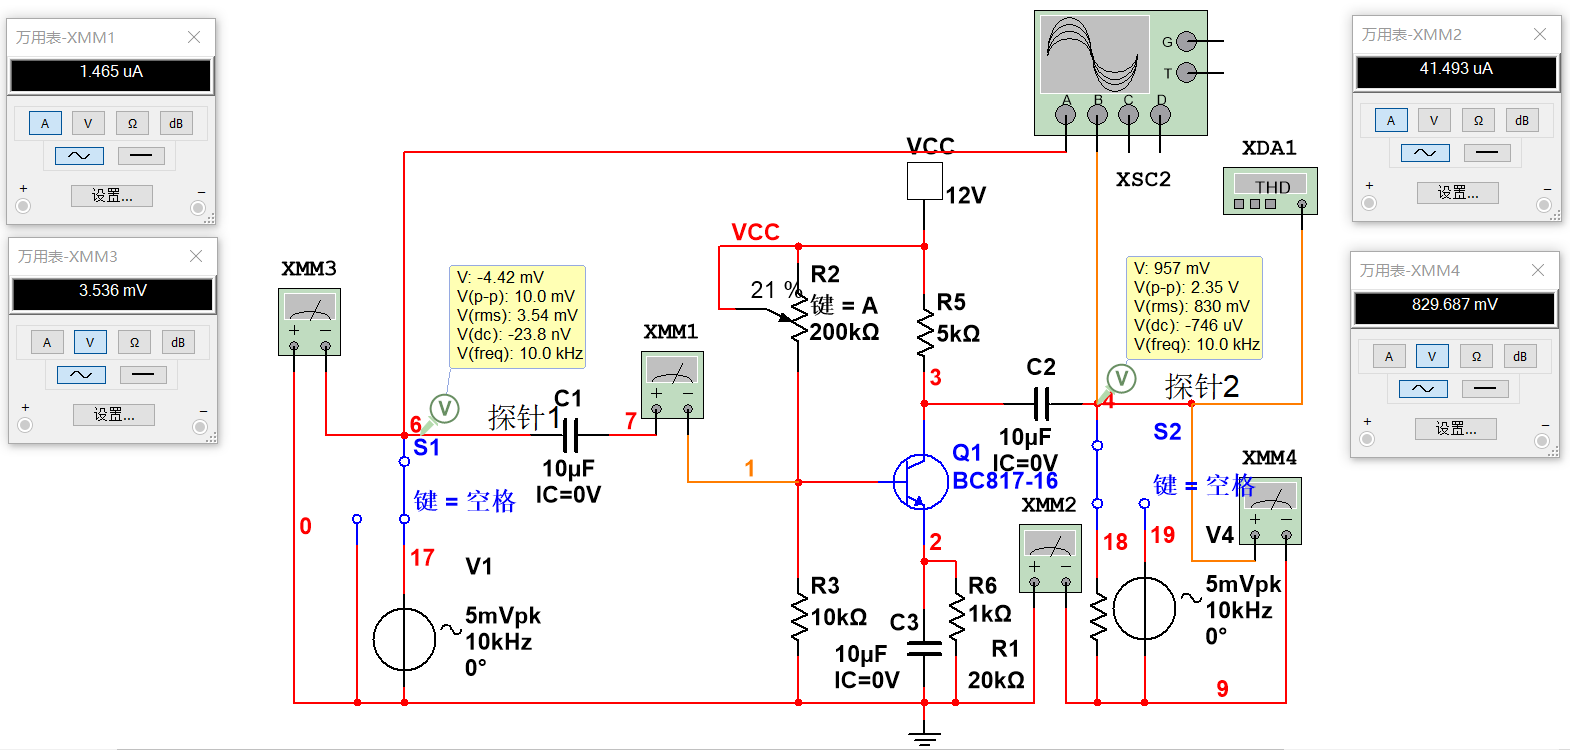
\includegraphics[width=0.8\linewidth]{1/Ri.png}
	\caption{单级放大电路原理图}
	\label{fig:单级放大电路原理图}
\end{figure}

单级放大电路原理图如图\ref{fig:单级放大电路原理图}所示,采用分压式偏置电路,有效稳定静态工作点。

其中$ R_3, R_2 $为偏置电阻,$ V_\mathrm{be} = \dfrac{R_2}{R_2 + R_3} V_\mathrm{cc} $,通过调节$ R_2 $阻值大小可以改变$ V_\mathrm{be} $进而改变静态工作点;

$ R_6 $具有直流负反馈作用,帮助稳定静态工作点,而$ C_3 $则是在交流通路中将$ R_6 $短路,增大电路放大倍数;

$ C_1, C_2 $都是耦合电容,隔直通交,其中$ C_1 $是避免交流小信号影响静态工作点,C2是滤除直流信号,避免静态工作点影响输出信号。

\subsection{指标计算}%
\label{sub:\arabic{chapter}指标计算}

\begin{figure}[H]
	\centering
	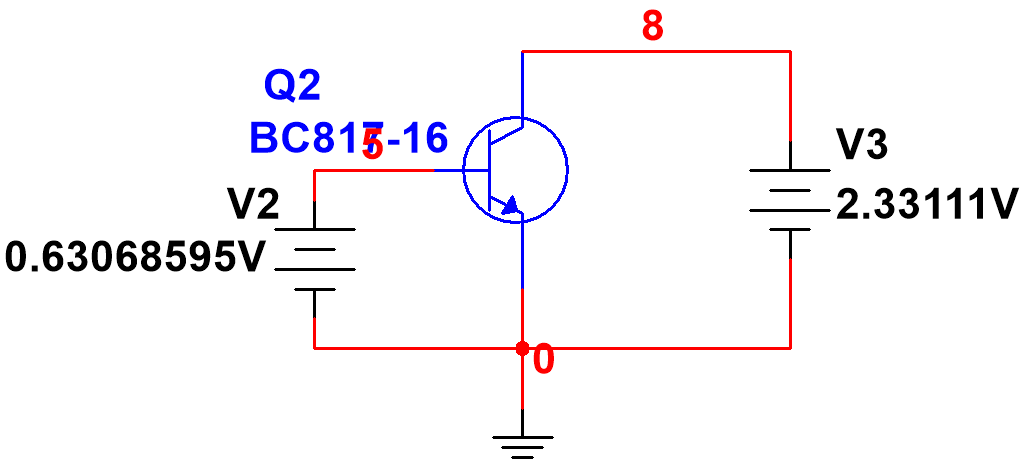
\includegraphics[width=0.8\linewidth]{1/measure.png}
	\caption{测量}
	\label{fig:测量}
\end{figure}

\begin{figure}[H]
	\centering
	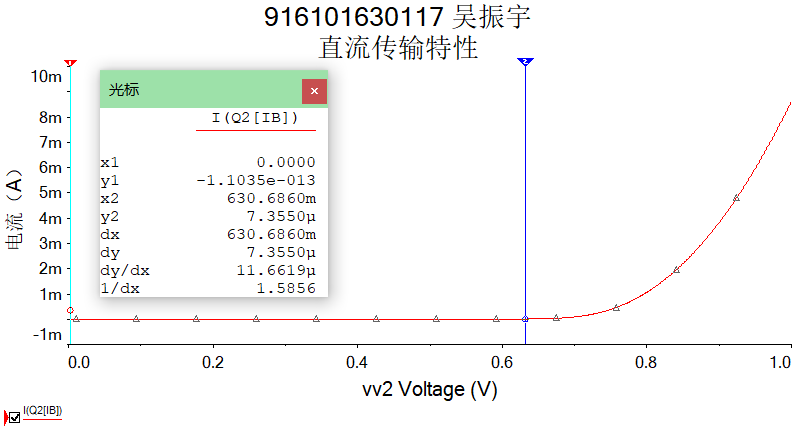
\includegraphics[width=0.8\linewidth]{1/input.png}
	\caption{输入特性曲线}
	\label{fig:输入特性曲线}
\end{figure}

\begin{figure}[H]
	\centering
	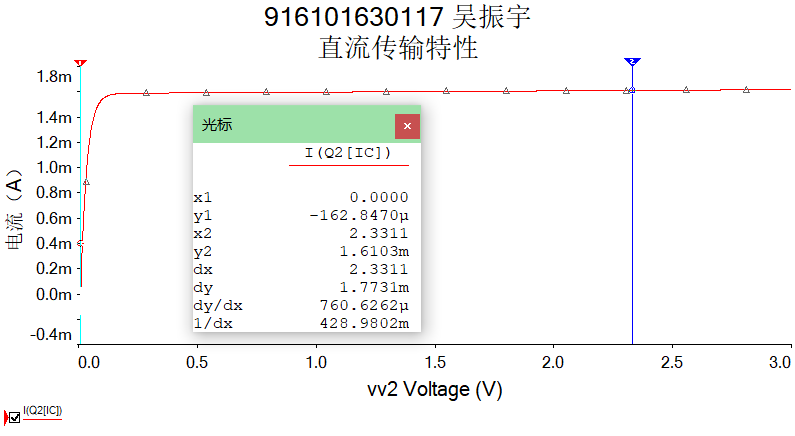
\includegraphics[width=0.8\linewidth]{1/output.png}
	\caption{输出特性曲线}
	\label{fig:输出特性曲线}
\end{figure}

根据要求,输出电阻决定了图\ref{fig:单级放大电路原理图}中$ R_5 $为\SI{5}{\kohm}。其它参数选取适当。

\subsection{仿真结果}%
\label{sub:\arabic{chapter}仿真结果}

\begin{table}[H]
	\centering
	\caption{单级放大电路失真指标}
	\label{tab:单级放大电路失真指标}
	\csvautobooktabular{tab/1/1-1.csv}
\end{table}

\begin{table}[H]
	\centering
	\caption{三极管参数}
	\label{tab:三极管参数}
	\csvautobooktabular{tab/1/1-2.csv}
\end{table}

\begin{table}[H]
	\centering
	\caption{单级放大电路参数}
	\label{tab:单级放大电路参数}
	\csvautobooktabular{tab/1/1-3.csv}
\end{table}

\subsubsection{饱和失真}%
\label{ssub:饱和失真}

饱和失真主要是将静态工作点调整至饱和区附近。

\begin{figure}[H]
	\centering
	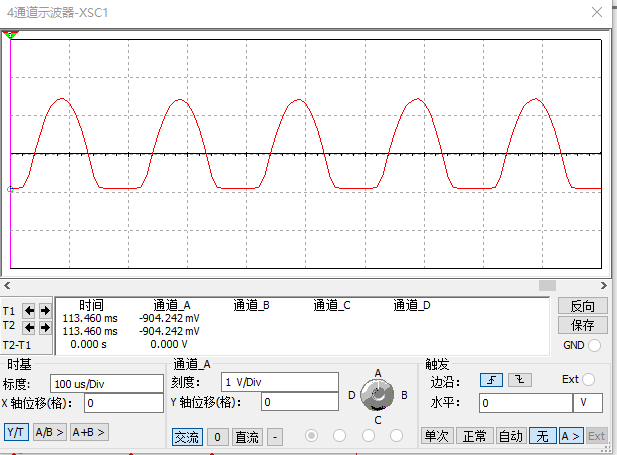
\includegraphics[width=0.8\linewidth]{1/saturation.png}
	\caption{单级放大电路饱和失真}
	\label{fig:单级放大电路饱和失真}
\end{figure}

饱和失真波形如图\ref{fig:单级放大电路饱和失真}所示,由于是反相放大器,所以饱和失真削弱了下半周期,出现削平波形。

\subsubsection{截止失真}%
\label{ssub:截止失真}

截止失真主要是将静态工作点调整至截止区附近,同时注意不能太靠近截止区,否则放大倍数受影响,失真波形不明显。

\begin{figure}[H]
	\centering
	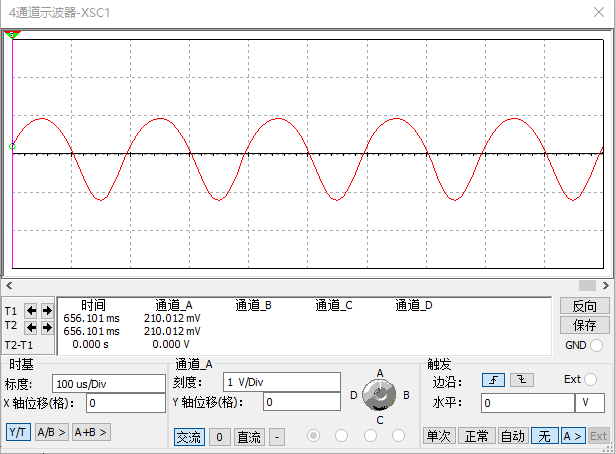
\includegraphics[width=0.8\linewidth]{1/cutoff.png}
	\caption{单级放大电路截止失真}
	\label{fig:单级放大电路截止失真}
\end{figure}

截止失真波形如图\ref{fig:单级放大电路截止失真}所示,由于是反相放大器,所以饱和失真削弱了上半周期,出现削平波形。

\subsubsection{最大不失真}%
\label{ssub:最大不失真}

最大不失真主要是将静态工作点调整至放大区中间,即能够实现最大不失真信号幅度的测量。

主要方法是先调节到恰好饱和失真、截止失真,测量静态工作点电压并取其平均值即为最大不饱和失真静态工作点附近;再通过细微调整确定最大不失真静态工作点以及输出幅值。

图\ref{fig:输出特性曲线}为BC817-16管输出特性曲线,通过比较交流负载线与输出特性曲线交点可知理论上最大不失真静态工作点$ V_\mathrm{ce} $约为\SI{3.7}{\V}左右,与实验所得结果\SI{3.95}{\V}吻合。

\begin{figure}[H]
	\centering
	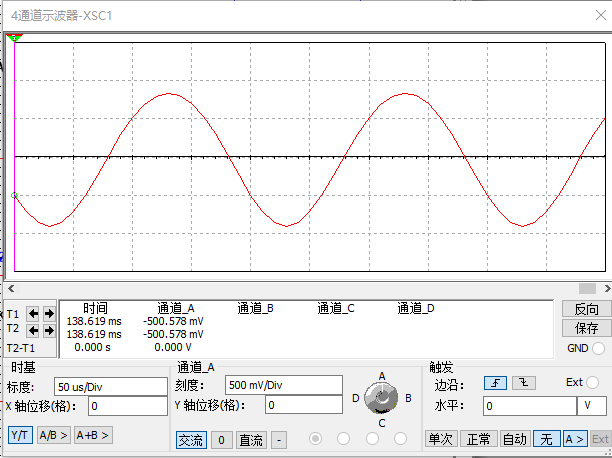
\includegraphics[width=0.8\linewidth]{1/normal.png}
	\caption{单级放大电路最大不失真}
	\label{fig:单级放大电路最大不失真}
\end{figure}

图\ref{fig:单级放大电路最大不失真}即最大不失真输出波形,其中输入电压峰值\SI{5}{\mV},输出电压峰值1.6V左右。上半周期波形峰值略小于下半周期波形,这是由于输出特性曲线靠近截止区时曲线略有上移引起的非线性失真,属于正常情况。

\subsubsection{单级放大电路输入电阻}%
\label{ssub:单级放大电路输入电阻}

如图\ref{fig:单级放大电路原理图}所示即为输入电阻测量电路,即断开输出电阻,输入端添加一个信号源。

\subsubsection{单级放大电路输出电阻}%
\label{ssub:单级放大电路输出电阻}

如图\ref{fig:单级放大电路输出电阻}所示即为输出电阻测量电路,即短路输入端电压源,输出端断开输出电阻,添加一个信号源。

\begin{figure}[H]
	\centering
	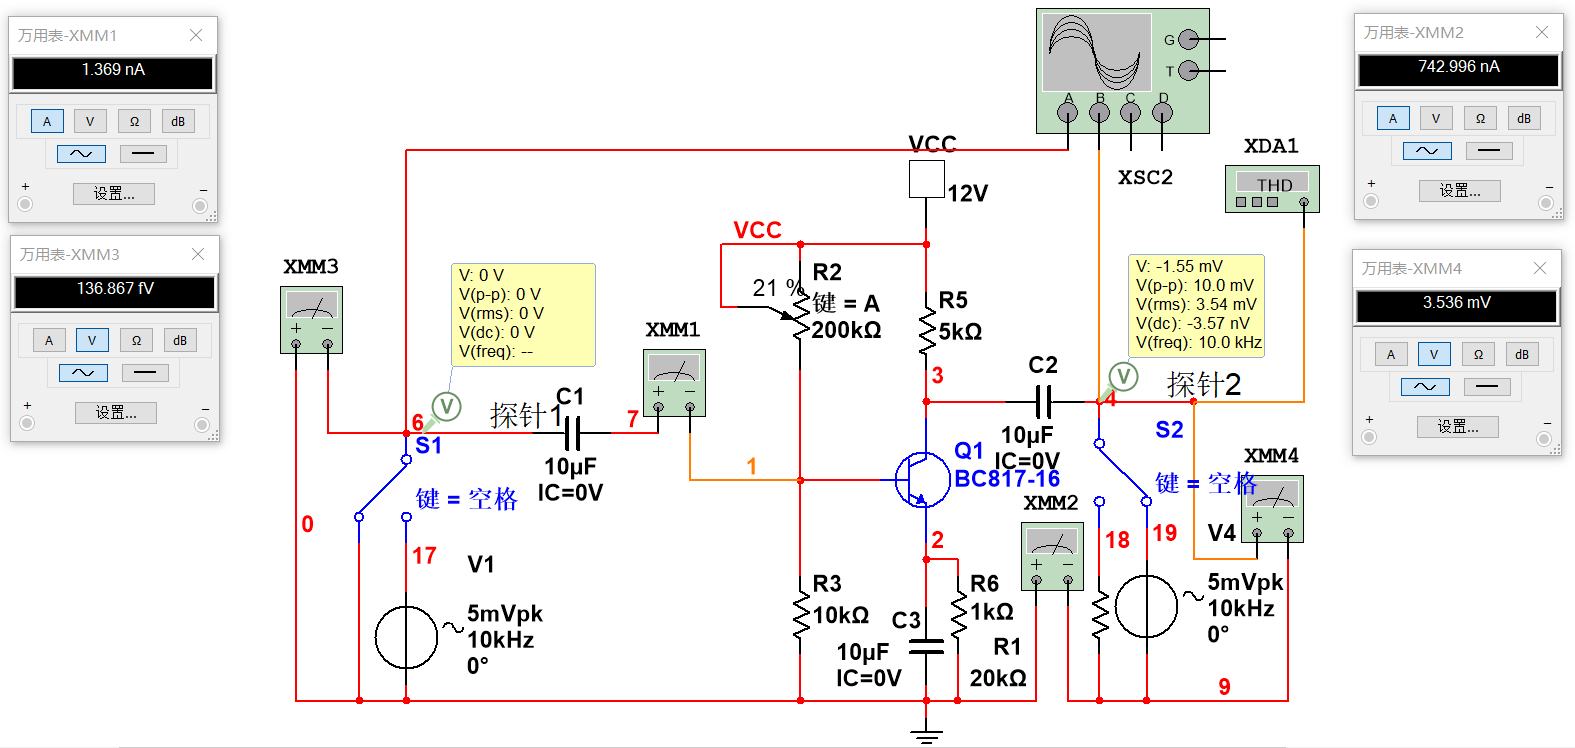
\includegraphics[width=0.8\linewidth]{1/Ro.png}
	\caption{单级放大电路输出电阻}
	\label{fig:单级放大电路输出电阻}
\end{figure}

\subsubsection{频率响应}%
\label{ssub:频率响应}

频率响应原理图如图\ref{fig:单级放大电路原理图}所示,其中信号源峰值\SI{5}{\mV},频率\SI{10}{\kHz}。

采用交流分析时添加公式$ V(3)/V(1) $即为放大倍数,注意单位选为\SI{}{\dB}。

如图\ref{fig:单级放大电路增益}中频增益为\SI{41.43}{\dB},中频增益减\SI{3}{\dB}即为上下限增益数值,对应即为上下界频率。

\begin{figure}[H]
	\centering
	\begin{subfigure}[H]{.8\linewidth}
		\centering
		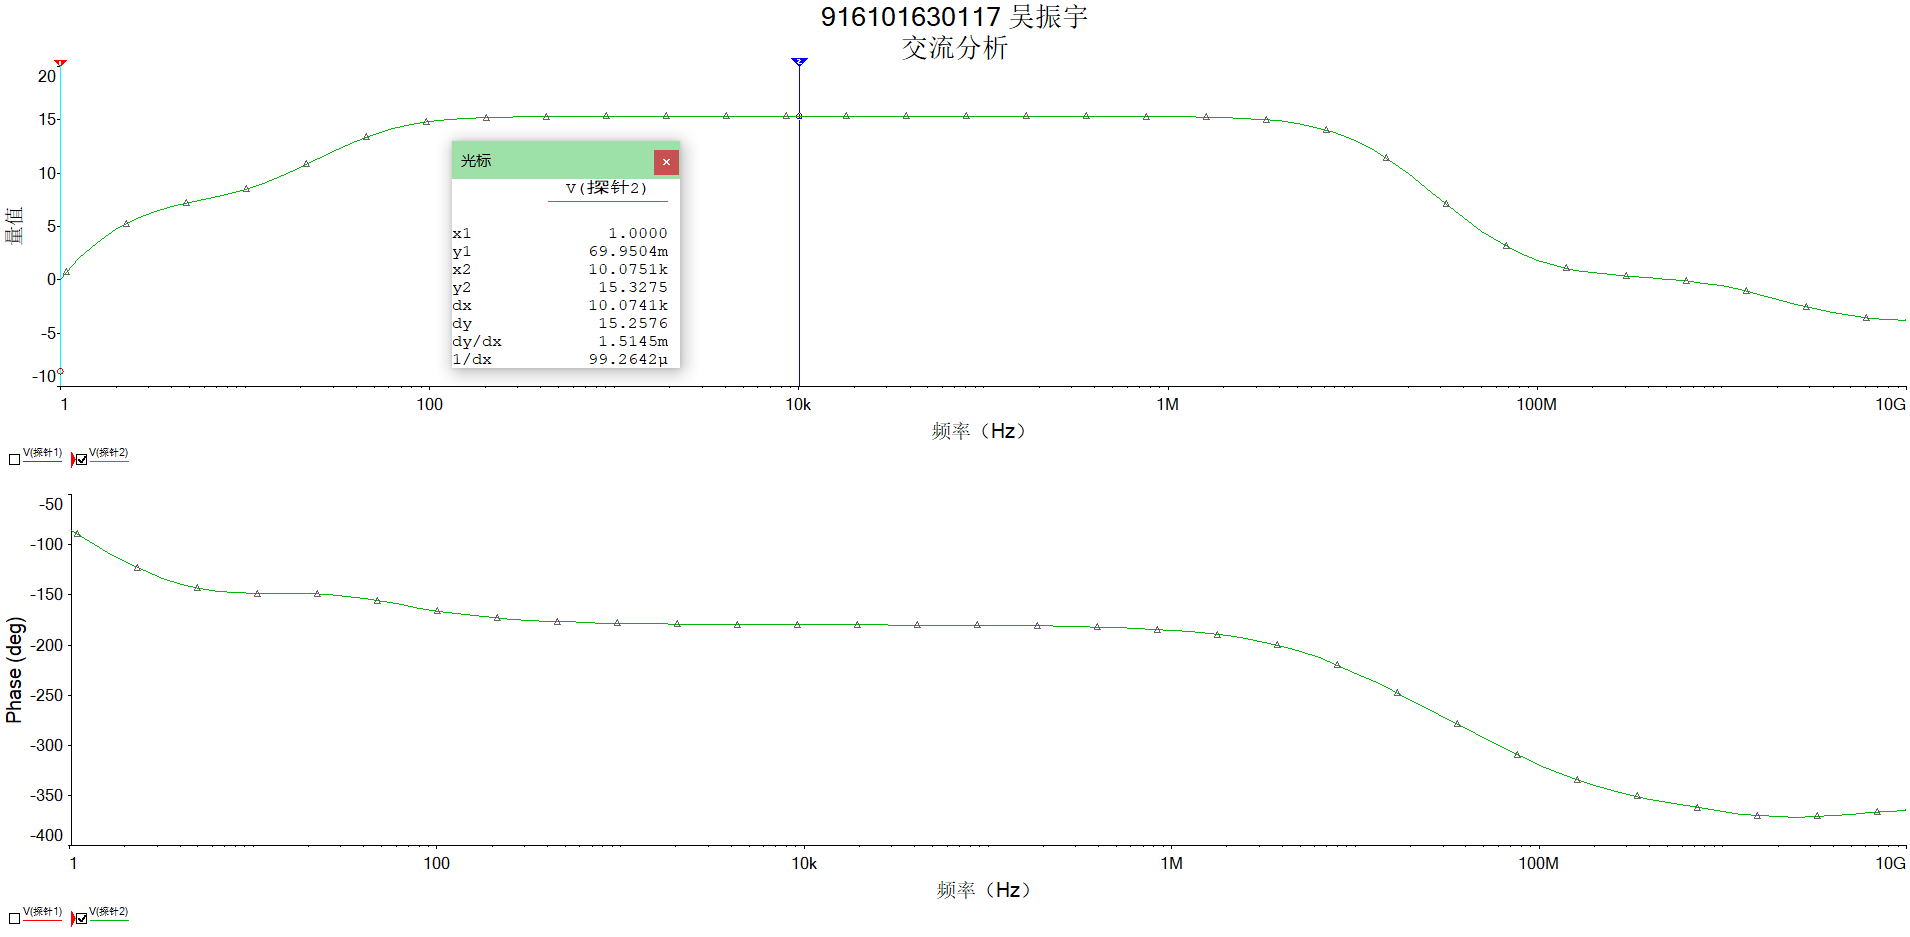
\includegraphics[width=\linewidth]{1/f.png}
		\caption{单级放大电路中频增益}
		\label{fig:单级放大电路中频增益}
	\end{subfigure}
	\quad
	\begin{subfigure}[H]{.8\linewidth}
		\centering
		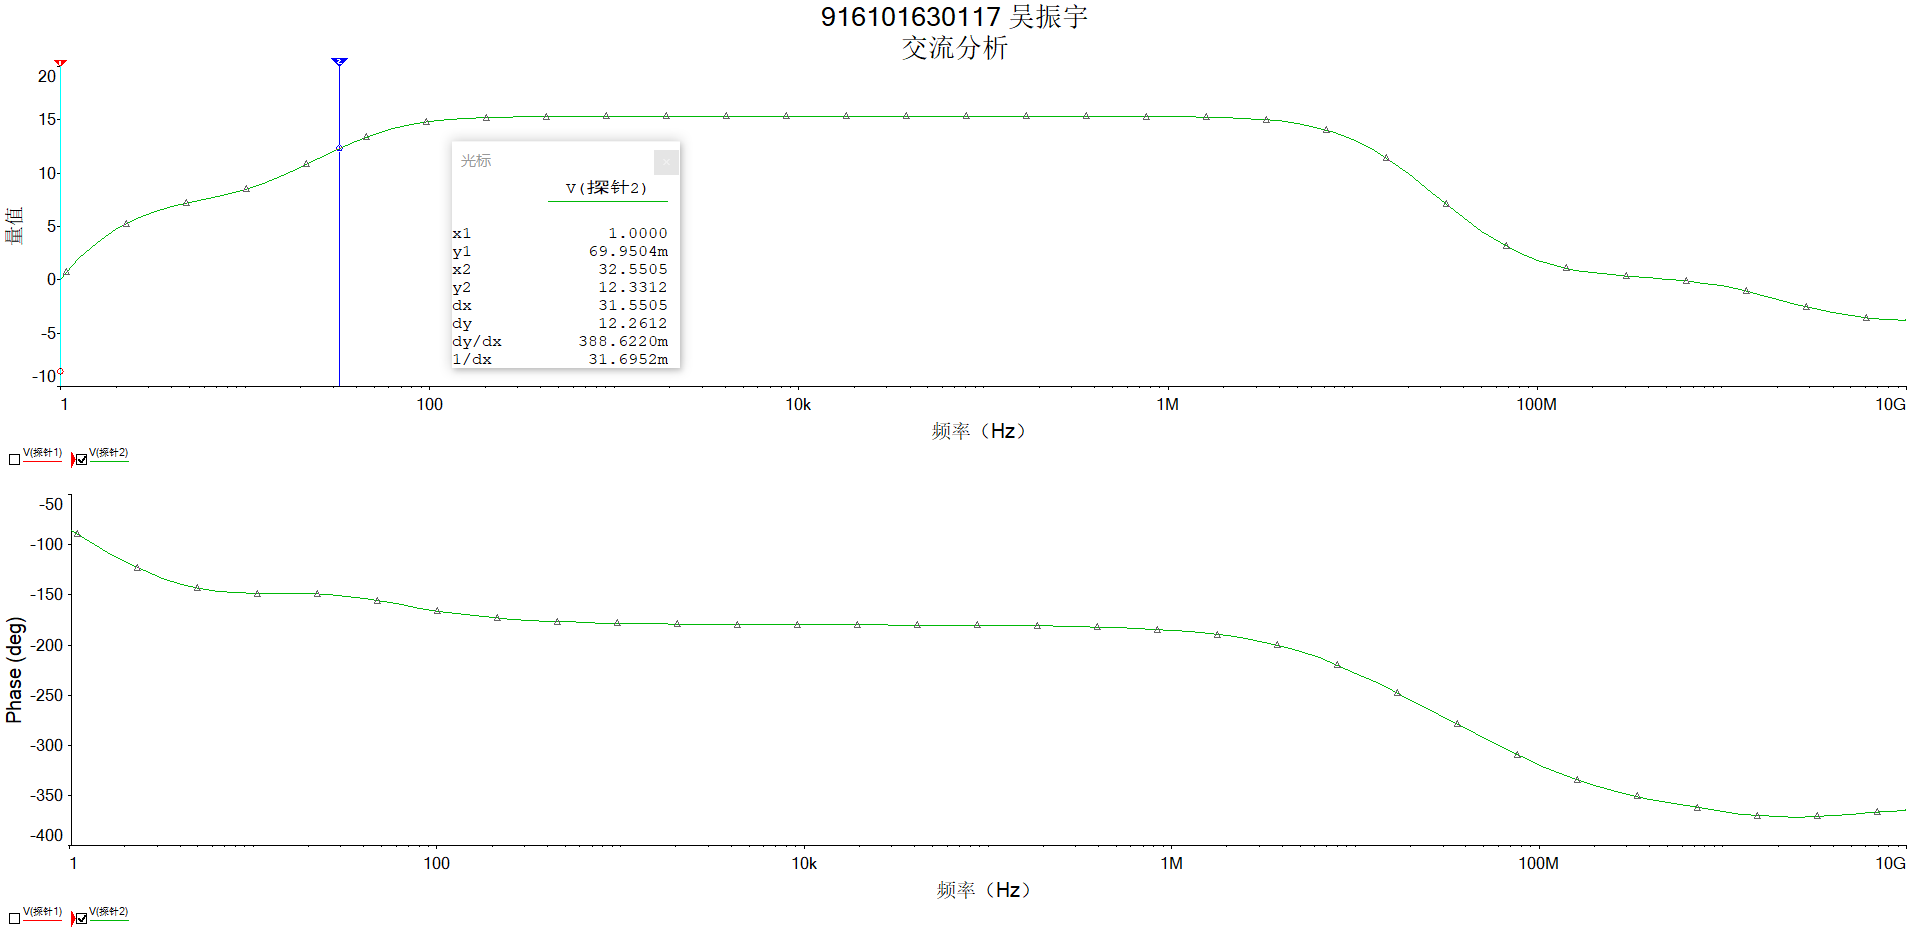
\includegraphics[width=\linewidth]{1/fL.png}
		\caption{单级放大电路下限增益}
		\label{fig:单级放大电路下限增益}
	\end{subfigure}
	\quad
	\begin{subfigure}[H]{.8\linewidth}
		\centering
		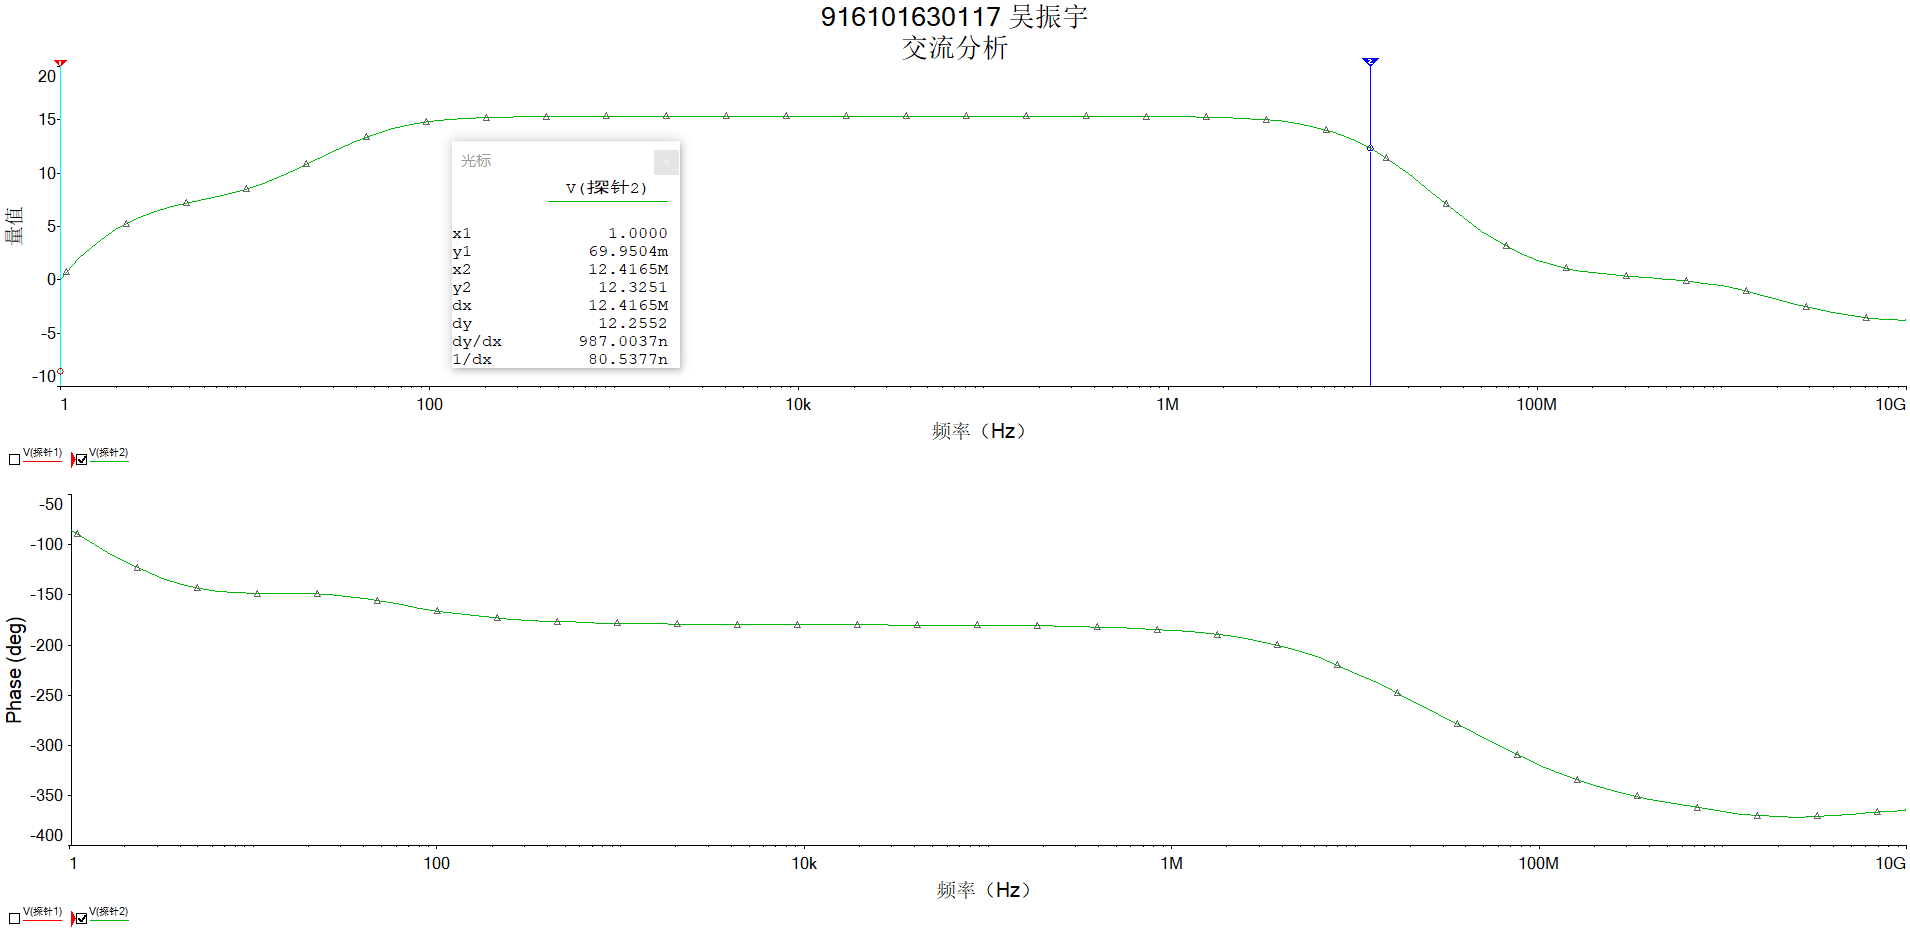
\includegraphics[width=\linewidth]{1/fH.png}
		\caption{单级放大电路上限增益}
		\label{fig:单级放大电路上限增益}
	\end{subfigure}
	\caption{单级放大电路增益}
	\label{fig:单级放大电路增益}
\end{figure}

\subsection{误差分析}%
\label{sub:\arabic{chapter}误差分析}

\subsubsection{输入电阻误差分析}%
\label{ssub:输入电阻误差分析}

采用交流分析法测量输入电阻,图\ref{fig:输入交流通路}为输入交流通路。由图可知输入电阻理论值为$ (R_2+R_3)\parallel R_5\parallel r_\mathrm{be} $

\begin{figure}[H]
	\centering
	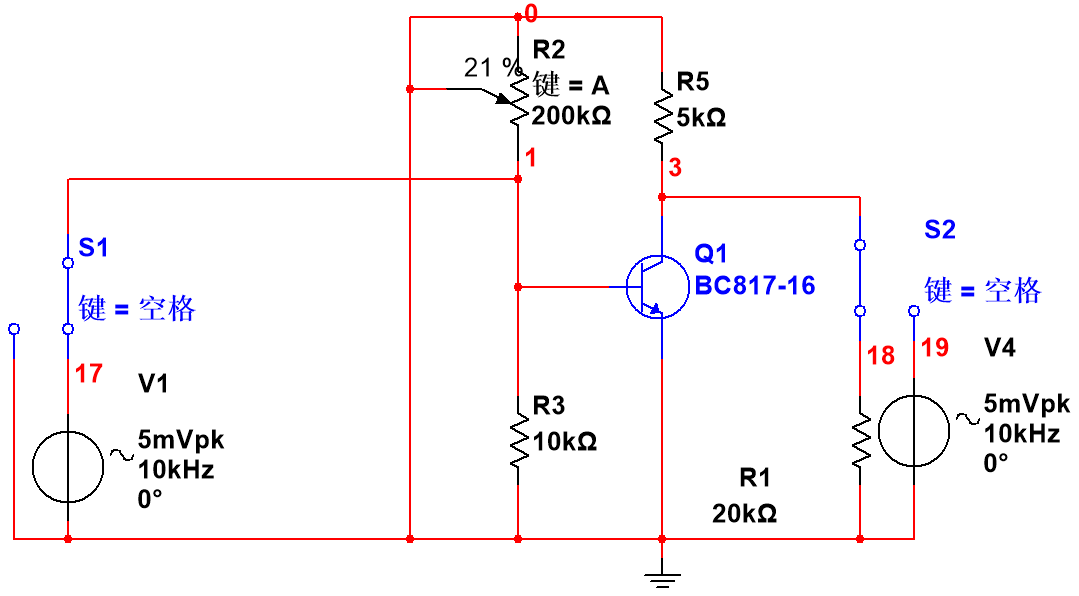
\includegraphics[width=0.8\linewidth]{1/RiAC.png}
	\caption{输入交流通路}
	\label{fig:输入交流通路}
\end{figure}

其中$ r_\mathrm{be} = \dfrac{\SI{26}{\mV}}{\SI{7.35384}{\uA}} + \SI{200}{\ohm} = \SI{3.735569}{\kohm} $,理论输入电阻约为\SI{2.38}{\kohm},与实验测得数据\SI{2.413652}{\kohm}基本一致。

\subsubsection{输出电阻误差分析}%
\label{ssub:输出电阻误差分析}

采用交流分析法测量输出电阻,图\ref{fig:输入交流通路}为输出交流通路。由图可知输入电阻理论值为$ R_5 $

\begin{figure}[H]
	\centering
	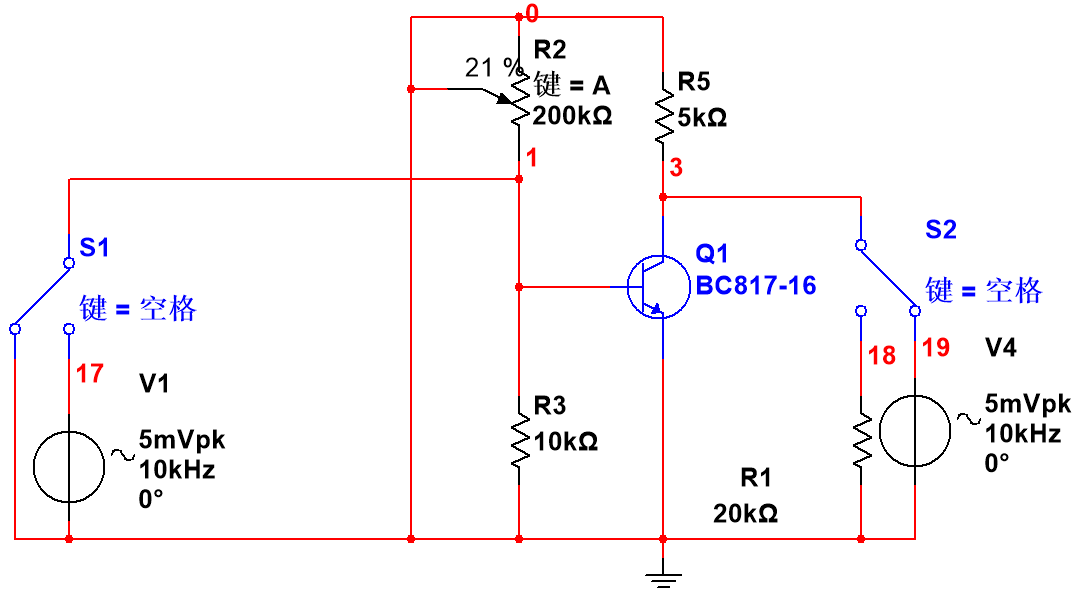
\includegraphics[width=0.8\linewidth]{1/RoAC.png}
	\caption{输出交流通路}
	\label{fig:输出交流通路}
\end{figure}

输出电阻理论值为$ R_5 $ ,为\SI{5}{\kohm}。与实验测得数据\SI{4.75911}{\kohm}基本一致。

\section{实验小结}%
\label{sec:\arabic{chapter}实验小结}

单级放大电路是所有放大电路的基础。难度并不算大,但熟练掌握为之后的学习做好了良好
的铺垫。

